% ===================================================================================
% Methodology redraft -- 2026-08-22, v2. Structure, section/subsection names, paragraph
% breaks and equation labels match the user's own current draft exactly (kept
% deliberately unchanged, per instruction) -- only the WORDING is edited, applying the
% reviewer feedback below, each checked against code before being applied rather than
% taken on faith.
%
% Applied as-suggested (verified sound):
%   1. Q1's target restated as height POSITION, not growth rate.
%   2. "Two-stage" now describes Q1's whole procedure (extract target, then model it),
%      not the mixed-effects model itself -- table entry and lead sentence both fixed.
%   3. Random-intercept explanation corrected: a fitted intercept per compartment PLUS
%      one shared variance sigma_u^2 -- not "one variance number", and not implied to
%      identify microclimate/soil specifically.
%   4. Pooled-metric vs. fold-mean-SD conflict reconciled -- both ARE used in this
%      project (confirmed against TEMP result tables earlier this session), for
%      different purposes; now stated as such instead of silently contradicting.
%   6. Coefficients vs. SHAP: now states conclusions are compared, not raw values.
%   7. Q2's opening no longer states Q1's finding as settled fact before Results.
%   8. GNNWR equation target made explicit: Delta-y-hat_max, not generic y-hat_i.
%   9. "Does not affect the R^2 comparison" (an unsafe absolute claim) replaced with a
%      cautious statement -- both predictive performance AND local coefficients need
%      careful reading, not just the coefficients.
%   11. Asymptote-parameterisation citation sentence added.
%   12. One-sentence Q2 model-comparison summary added.
%
% Checked against code/data before applying (reviewer's item was a claim ABOUT the
% implementation -- verified rather than assumed):
%   5. Held-out mixed-model prediction: `models/spatial_attribution/nlme.py` has NO
%      `.predict()` call anywhere, and is only ever invoked by
%      `run_rq1_attribution.py` for `fixed_effects_table()` (coefficients) and
%      `variance_explained_by_fixed_effects()` (a variance-decomposition stat) -- this
%      project's LMM is NEVER used to generate held-out predictions on unseen
%      compartments, so there is no "fixed-effects-only" prediction step to describe.
%      Written to say that plainly instead of adding a sentence implying a prediction
%      step that doesn't exist.
%   10. p4/p5 wording: `data_processing/export_growth_curve_tables.py` comment confirms
%       p1-p5 form a per-plot recorded tuple (7 distinct value-sets total in this data),
%       tied to species/region, "not tied to that plot's own yldc" -- i.e. NOT something
%       that varies by yield-class value. The reviewer's safer wording ("fixed at their
%       published values for the corresponding Forest Research curve") is accurate;
%       adopted.
%
% NOT applied, with reasons:
%   - "Remove XGBoost gain, keep only SHAP" -- Q2's own results text (already in this
%     chapter's Results section) explicitly cites "three converging attribution
%     metrics: Elastic Net coefficients, XGBoost gain importance, and SHAP values" --
%     gain is load-bearing for an existing results claim, not redundant. Kept.
%   - "Move clearfell/measurement-error rules to the Data chapter" -- plausible, but no
%     existing home for these exact rules was confirmed in the Data chapter before this
%     file was written. Flagged in chat for a decision, not silently relocated.
% ===================================================================================

%=======================================================================================
%=======================================================================================
\chapter{Methodology and Experimental Framework} \label{ch:methodology}
\section{Experimental framework}
Q1 attributes a plot's deviation from the baseline growth curve to environmental and management factors. Q2 tests whether spatially varying relationships capture what global models miss. Finally, Q3 evaluates whether these signals improve top-height predictions.

\begin{table}[!ht]
\centering
\footnotesize
\renewcommand{\arraystretch}{1.15}
\begin{tabularx}{\linewidth}{@{} l >{\raggedright\arraybackslash}X >{\raggedright\arraybackslash}X >{\raggedright\arraybackslash}X @{}}
\toprule
Q & Unit and target & Models or comparison & Main evaluation \\
\midrule
Q1 & Plot; mean pooled-CR residual & Elastic Net, XGBoost and linear
mixed-effects model & Spatial block CV (Elastic Net, XGBoost); LMM coefficients and variance decomposition; residual Moran's $I$ \\
Q2 & Plot; difference between fitted and yield-class-implied asymptotes & Elastic Net, XGBoost
and GNNWR & Five-fold spatial block CV; attribution, Moran's $I$ and target audit \\
Q3 & Plot--survey row; 95th-percentile top height, and row-level error reduction against the
fold-matched CR curve & CR, linear regression, random forest, XGBoost, DNN, PINN and PINN-$k$
& Five-fold spatial block CV; random-split and PINN forward-pass diagnostics; CR-error-quartile
correction with permutation control \\
\bottomrule
\end{tabularx}
\caption{\small{Units, targets and evaluation used for each question. Q3's row-level CR-error-quartile
check reuses Q3's own model predictions (conditioned DNN, PINN, PINN-$k$ and XGBoost) rather
than introducing a separate comparison.}}
\label{tab:rq-framework}
\end{table}

\paragraph*{Data partitions and leakage control}
The four-survey cohort served as the main dataset, while the six-survey cohort was kept as a longer-term sensitivity check. For Q1 and Q2, each plot had one summary value, while Q3 used every plot-survey row.

Spatial-block cross-validation prevented data leakage by assigning whole forest compartments to folds, ensuring no compartment appeared in both training and testing \cite{roberts2017Cross_C5_EVAL}. Training plots within 60\,m of validation or test plots were also removed to prevent spatial spillover. Five folds of roughly equal size were created. In each round, three folds trained the model, one fold tuned it, and one fold tested it. Each compartment was tested exactly once, and all test predictions were combined to calculate final performance metrics \cite{ploton2020Spatial_C5_EVAL}.


\begin{figure}[!htbp]
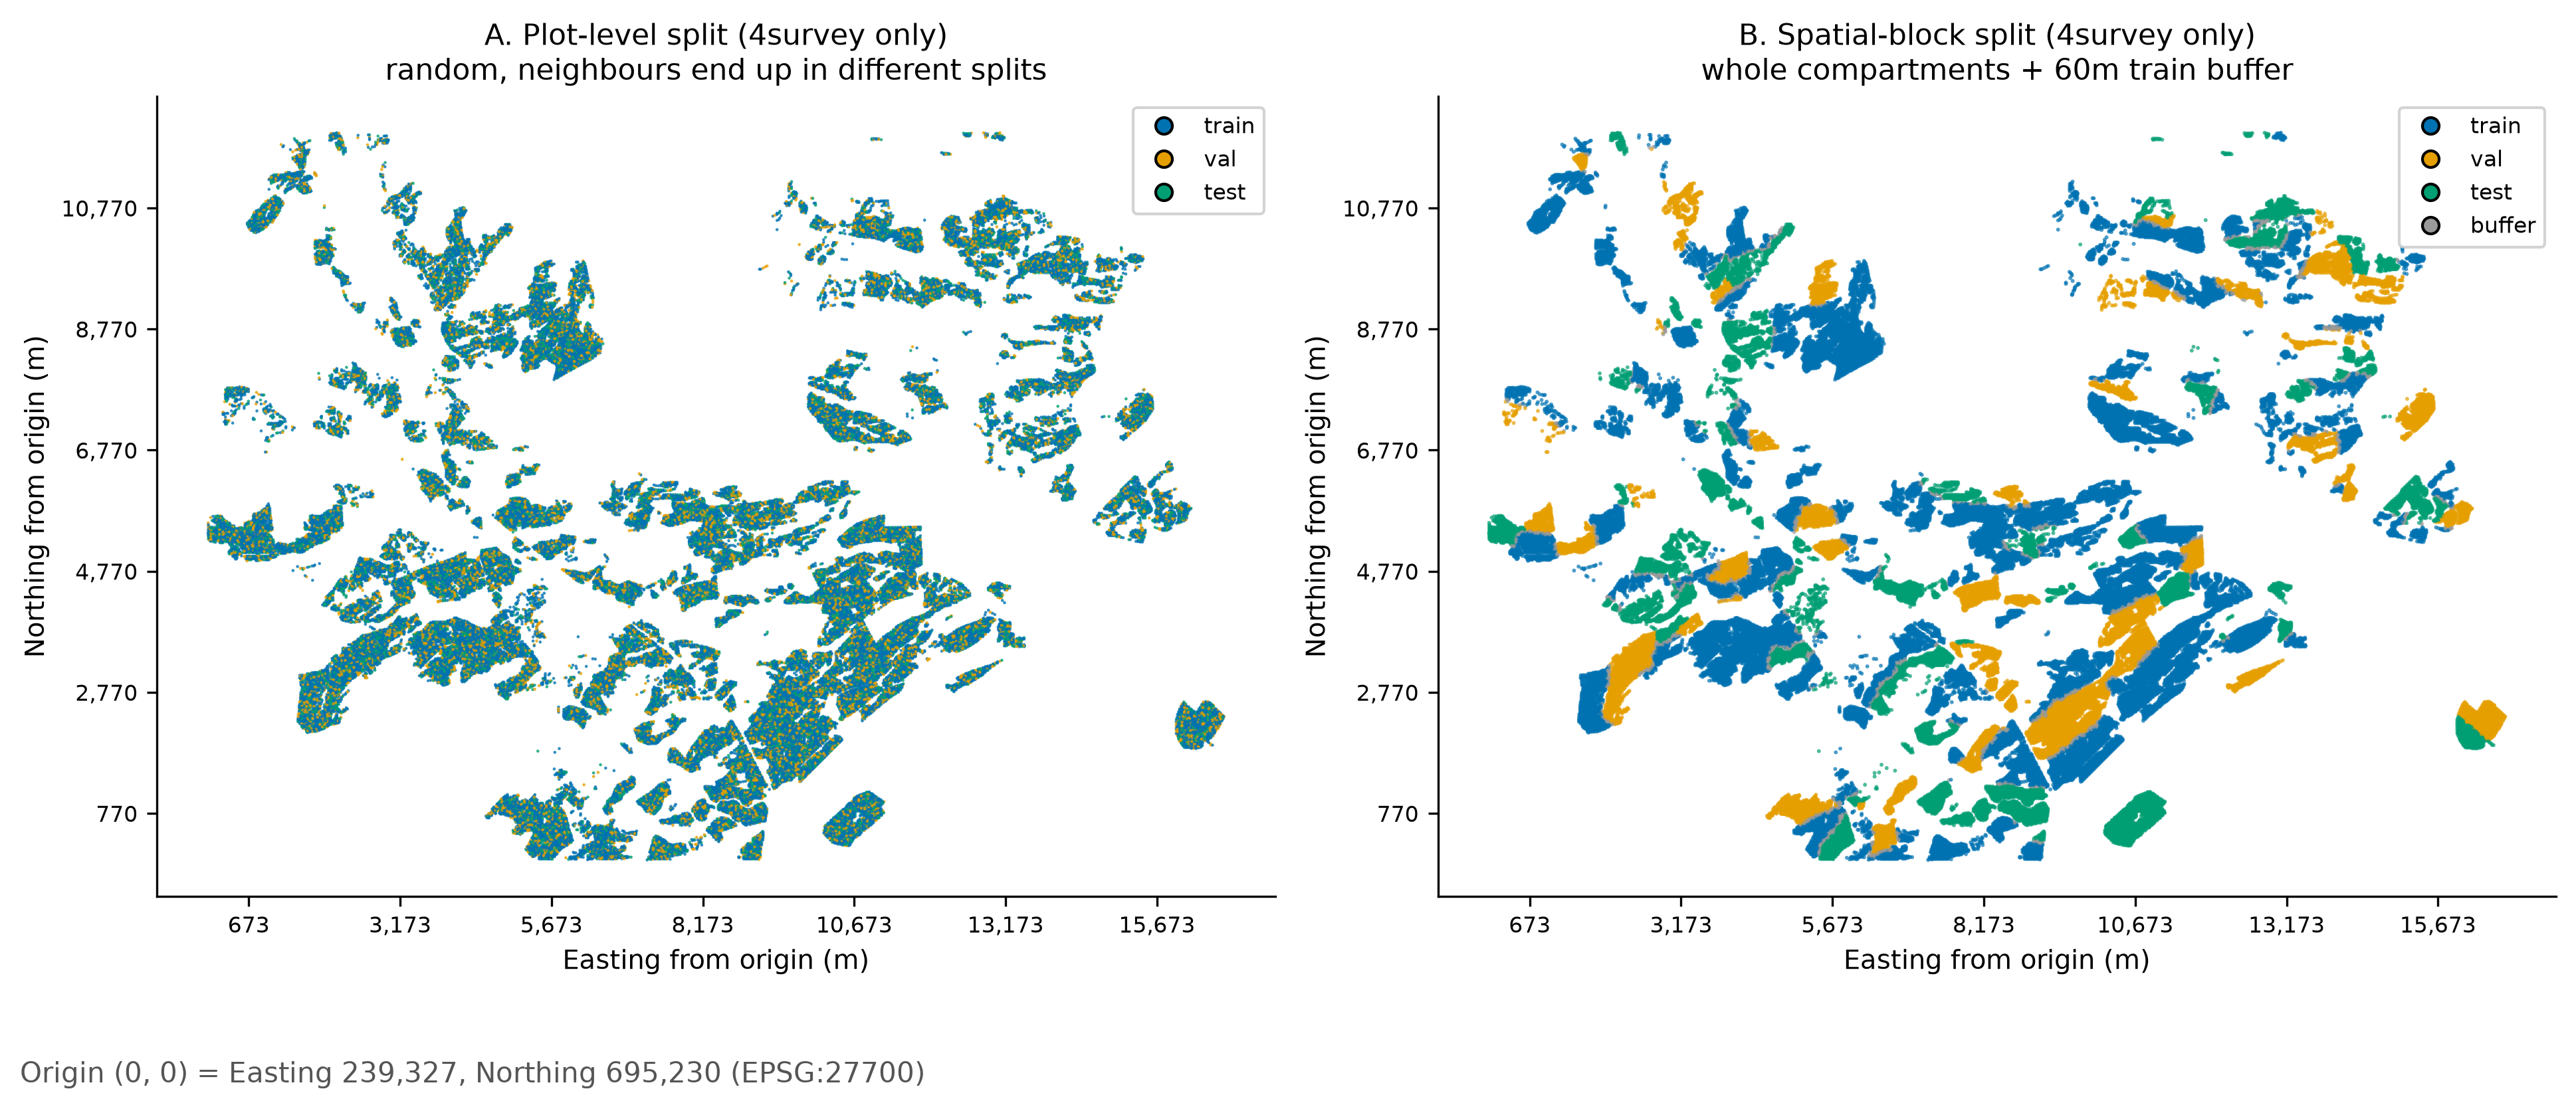
\includegraphics[width=1.0\textwidth]{figures/fig_methodology/fig_method_map_splits.png}
\centering
\caption{\small{Evaluation data-splitting strategies: (A) random plot-level split and (B) compartment-level spatial-block split with a 60\,m buffer.}}
\label{fig:splits-combined}
\end{figure} %TODO: increae font size. for axis.

Continuous variables were scaled using the training data and applied to the validation and test sets. Age was scaled on its own so PINN outputs could be turned into metres per year. Soil types were converted into binary categories. Compartment and block IDs were left out of the models. Two neighbour-height variables were also dropped because they were made using nearby plot heights before the split, which could leak test answers.

\section{Q1: Explaining growth deviations}
Q1 uses a two-stage analysis. First, repeated observations are reduced to one mean departure per plot. Second, Elastic Net, XGBoost and a linear mixed-effects model explain this target. The four-survey cohort is used because the six-survey cohort has too few compartments for spatial testing. Here, $i$ marks a plot, $t$ marks a survey, $H_{it}$ and $a_{it}$ are observed height and age, and $T_i$ is the number of surveys for plot $i$. $H(a)$ is the shared Chapman-Richards growth curve (Equation~\eqref{eq:cr}) at age $a$. Equation~\eqref{eq:cr-gap} computes the gap between measured height and the baseline curve, while Equation~\eqref{eq:mean-cr-residual} averages this gap over time to give one mean departure per plot:
\begin{align}
r_{it} &= H_{it} - H(a_{it}), \label{eq:cr-gap} &
\bar{r}_i &= \frac{1}{T_i} \sum_{t=1}^{T_i} r_{it}. \label{eq:mean-cr-residual}
\end{align}
Positive $\bar{r}_i$: observed top height lies above the baseline on average. Negative: below. The target measures average vertical position relative to the baseline, not directly a growth rate -- averaging does not imply the same sign held at every survey. Stand age is omitted from model predictors since the growth curve already accounts for it.

We test Elastic Net and XGBoost using five-fold spatial cross-validation. Elastic Net tunes its penalty parameters on each training fold using an inner loop. XGBoost uses tuned parameters (depth 4, learning rate 0.04, up to 500 trees with early stopping). Pooled out-of-fold metrics ($R^2$, RMSE, MAE) give the headline estimates for both models.

To account for plots grouped within compartments, we fit a linear mixed-effects model, fit independently on each fold's own training partition (never on held-out data, and never used to predict an unseen compartment):
\begin{equation}
\bar{r}_i = \beta_0 + \boldsymbol{\beta}^{\top}\mathbf{x}_i + u_{c[i]} + \varepsilon_i, \qquad u_c \sim \mathcal{N}(0, \sigma_u^2).
\label{eq:mixed-effects}
\end{equation}
$\boldsymbol{\beta}^{\top}\mathbf{x}_i$ represents fixed effects (landscape-wide relationships reported across all plots, such as slope or TOPEX). $u_{c[i]}$ is the random intercept for plot $i$'s compartment: each training compartment receives its own fitted intercept, drawn from a shared distribution with variance $\sigma_u^2$ -- that variance describes how much intercepts vary between compartments overall, it is not itself a random quantity. These effects capture unexplained compartment-level grouping, not its ecological cause -- the model does not identify microclimate, soil, or any other specific mechanism. This model is used only for its fitted coefficients and for the variance-explained comparison below.

Parameters ($\boldsymbol{\beta}$ and $\sigma_u^2$) are fitted using restricted maximum likelihood (REML), which avoids the slight variance underestimation seen in standard maximum likelihood (ML). However, when directly comparing models with different fixed effects to assess how much compartment variance the environmental predictors explain, ML is used instead, as REML likelihoods cannot be compared across different fixed-effect structures. Because the mixed-effects model is refit independently on each fold's training partition, its coefficients are also reported as mean $\pm$ standard deviation across folds -- a genuine measure of fold-to-fold variation, not a single full-data fit. This is a different summary from Elastic Net and XGBoost's pooled out-of-fold metrics above: pooled metrics are headline held-out accuracy figures; the mixed-effects model's mean $\pm$ SD describes how stable its in-sample coefficients are across spatial splits, not held-out accuracy.

Two concerns motivate four sensitivity checks; first, because canopy cover and top height come from the same LiDAR flights, a strong canopy-cover effect might reflect measurement overlap rather than true stand structure. We test this through three steps: (1) refitting Set~4 without canopy cover to assess the change in $R^2$; (2) checking direct correlations between canopy cover and each target; and (3) recalculating SHAP values without canopy cover to see if other predictors absorb its explanatory role.

Second, differences in terrain coefficients (such as slope and TOPEX) between Elastic Net and the mixed-effects model could reflect local, compartment-specific effects that global models miss. We test this with a fourth check: (4) measuring how much variance in slope and TOPEX occurs between compartments versus within them, identifying whether their spatial structure masks local relationships.

Elastic Net coefficient signs and selection, mixed-model fixed-effect signs, and XGBoost mean $|$SHAP$|$ rankings are compared for agreement on which variables matter and in what direction -- their raw magnitudes are not directly comparable, since each reflects a different kind of model, and mean $|$SHAP$|$ itself carries no sign. This comparison provides three complementary perspectives on growth drivers; agreement across all three indicates an association is less dependent on model structure, not that it is causal. Residual Moran's $I$ tests for remaining spatial clustering (Section~\ref{sec:eval-robustness}).


%------------------------------------------------
\section{Q2: Spatial attribution}
Global models assume one environment--growth relationship across the study area. Q2 tests whether allowing this relationship to vary by location improves explanation and reduces residual spatial clustering. We use GNNWR \cite{du2020Geographically_C6_GWR}, which uses a neural network to learn spatial weighting from geographic coordinates without fixing a rigid neighbourhood size.

However, GNNWR assumes local relationships are linear. If the true biological response is non-linear, fluctuating local coefficients may simply show that a straight line fits poorly in that area, rather than a real geographic difference in growth drivers. Coefficient variation may therefore indicate genuine spatial non-stationarity or a poor local approximation of a non-linear response; both predictive performance and individual local coefficients need careful, cautious reading, not just the coefficients on their own.

\paragraph*{What Q2's target actually measures:} For each plot, does its own growth so far point toward a higher or lower height ceiling than its assigned yield class predicts? $p_1$--$p_5$ are Forest Research's own published numbers that convert a yield-class rating into a full growth curve for a species and region; this project did not derive them, only reused them. $p_1$--$p_3$ and $p_4$--$p_5$ control different parts of the same sigmoid, not two competing curves -- the yield-class-implied curve is:
\begin{equation}
H^{\mathrm{yldc}}_i(a) = \underbrace{\left(\mathrm{yldc}_i\, p_{2,i}+p_{1,i}+2p_{3,i}\right)}_{\text{asymptote (ceiling)}} \cdot \underbrace{\left(1-e^{-p_{4,i}a}\right)^{p_{5,i}}}_{\text{shape (rate and curvature)}}.
\label{eq:yldc-full-curve}
\end{equation}
$p_4$ (growth rate) and $p_5$ (curve shape) are fixed at their published values for the corresponding Forest Research curve; only the height ceiling is allowed to differ from plot to plot. Environmental variation has previously been represented through the Chapman--Richards asymptote this way, supporting this as a parsimonious parameterisation rather than evidence that environmental effects act on this parameter alone \cite{scolforo2013Dominant_C2_CR}. For plot $i$ at survey $t$, splitting Equation~\eqref{eq:yldc-full-curve} into its two halves gives:
\begin{align}
g_{it} &= \left(1-e^{-p_{4,i}a_{it}}\right)^{p_{5,i}}, \label{eq:git-curve} \\
\hat y_{\max,i} &= \frac{\sum_t H_{it}g_{it}}{\sum_t g_{it}^2}, \label{eq:plot-ymax-fit} \\
y_{\max,i}^{\mathrm{yldc}} &= \mathrm{yldc}_i p_{2,i}+p_{1,i}+2p_{3,i}, \label{eq:yldc-asymptote} \\
\Delta y_{\max,i} &= \hat y_{\max,i}-y_{\max,i}^{\mathrm{yldc}}. \label{eq:local-ymax-diff}
\end{align}
With $p_4$ and $p_5$ fixed, Equation~\eqref{eq:plot-ymax-fit} has a closed-form least-squares estimate for $\hat y_{\max,i}$ -- this avoids estimating three correlated curve parameters from only 4--6 observations per plot. $\hat y_{\max,i}$ is the ceiling fitted from plot $i$'s own observed trajectory, while $y_{\max,i}^{\mathrm{yldc}}$ (Equation~\eqref{eq:yldc-asymptote}) is the ceiling implied by its assigned yield class, using that same fixed rate and shape. Their difference, $\Delta y_{\max,i}$ (Equation~\eqref{eq:local-ymax-diff}), is positive for a higher fitted ceiling than expected and negative for a lower one. $\hat y_{\max,i}$ is estimated, not observed; with rate and shape held constant, every real trajectory difference is forced into this one number.

Following the Q1 setup, Elastic Net and XGBoost are trained on $\Delta y_{\max}$ using Sets~2--4. Elastic Net tests a global linear relationship, XGBoost tests a global non-linear relationship, and GNNWR tests a spatially varying but locally linear relationship. Spatial variation is modelled using GNNWR via its Python library \cite{du2020Geographically_C6_GWR, du2022PyGNNWR_C6_GWR}:
\begin{equation}
\widehat{\Delta y}_{\max,i} = \beta_0(s_i) + \sum_j \beta_j(s_i) x_{ij}.
\label{eq:gnnwr}
\end{equation}
For each location $s_i$, GNNWR uses a neural network to learn spatial weights from distances to training plots; these weights determine the local coefficients $\beta_j(s_i)$, adjusting a global linear baseline. Each training fold's model uses only that fold's own training partition -- no fold sees another fold's data.

\subsection*{Computational adjustments and feature evaluation}
Full reference sets were used for headline GNNWR runs, after an early GPU memory limit forced a smaller, capped reference set in preliminary tests; the cap is kept only as its own later sensitivity check. Memory-intensive hat-matrix diagnostics were disabled: GNNWR AIC is approximated using raw feature counts rather than the true GWR-corrected effective degrees of freedom, and $F$-tests are not reported; predictive metrics ($R^2$, RMSE) are unaffected. Elastic Net and XGBoost were unaffected. %TODO: appendix section for full implementation detail not yet written.

Feature importance is assessed via XGBoost gain and test-fold SHAP values \cite{lundberg2017Unified_C7_XAI}, and GNNWR's own local coefficient distributions and maps.
Each feature group's contribution to $R^2$ is measured by permutation importance (shuffling that group's columns, no refit); its contribution to residual clustering is measured by removing the group from Set~4 and refitting, comparing Moran's $I$ before and after (4-survey cohort).

\subsection*{Target and outlier audit}
%TODO: flagged for a decision, not yet moved -- checked against data_processing/clean_master_data.py:
% no evidence found that these two rules are applied as general preprocessing elsewhere in
% this project; they appear specific to Q2's own plot-level asymptote-fitting population, which
% would make Methodology the correct home, not the Data chapter. Confirm before moving.
To remove bad data, plots are dropped if consecutive surveys match either rule:(1) Clearfell: Top height drops $\ge 25\%$, canopy cover drops $\ge 70\%$, and standing volume drops $\ge 70\%$.
(2) Measurement error: Top height drops $\ge 25\%$, while canopy cover drops $\le 10\%$ and volume does not drop. Plots with large height drops that match neither rule are kept. Extreme fitted ceilings ($\hat{y}_{\max,i}$) are identified using Tukey's $1.5\,\mathrm{IQR}$ rule \cite{tukey1977Exploratory_C5_EVAL}: % Tukey (1977) -- NB: mybibfile.bib has a near-duplicate entry (tukey1977exploratory_C5_EVAL, lowercase e) for the same book; dedupe before submission, this cites the capital-E one.
\begin{equation}
\left[Q_1 - 1.5\,\mathrm{IQR},\; Q_3 + 1.5\,\mathrm{IQR}\right].
\label{eq:tukey-fences}
\end{equation}
Fences are set separately per cohort following standard forest growth modelling practices \cite{weiskittel2011forest_C1_SS}. % Weiskittel et al. (2011)
Flagged plots are retained in primary runs, but evaluated in a sensitivity test by removing them from test predictions.

The audit checks if the top 1\% and 5\% largest residual plots overlap across Elastic Net, XGBoost, and GNNWR. We test their spatial distribution, distance to stand edges, wind shelter, and local coefficients against standard plots, and refit them without 2008 data, to assess whether extreme errors are associated with fitting artifacts, disturbance, or other environmental conditions -- these checks can flag an association, not establish a causal ecological trend. Which plots are flagged, and what that implies, is reported in Results.

%------------------------------------------------
\section{Q3: Prediction and physics guidance}

Q3 tests if environmental variables improve top-height predictions and evaluates physics-informed neural networks. Using five spatial folds on Set~3, we compare a baseline growth curve, standard tabular models, and neural networks, using the other feature sets to test the benefit of adding environmental data.

\subsection{Chapman--Richards (CR) baseline}
\begin{equation}
H(a) = y_{\max}\left(1 - e^{-ka}\right)^p,
\label{eq:cr}
\end{equation}
where $H(a)$ is height at age $a$, $y_{\max}$ is the height asymptote, $k$ is the growth rate, and $p$ controls curve shape. All three parameters are fit freely by non-linear least squares on each training fold and frozen, keeping test folds fully independent.

\subsection*{Conventional models}
We test three baselines: linear regression, random forest, and XGBoost \cite{chen2016XGBoost_C4_NN}. For Q3, XGBoost was tuned across 27 parameter settings over five folds using validation $R^2$ (Appendix~\ref{app:hyperparameters}).

\subsection{DNN and physics-informed models}
All neural networks use a three-layer trunk (128 units per layer, Leaky-ReLU) trained with Adam (learning rate $10^{-4}$, weight decay $10^{-5}$, batch size 256, early stopping). The standard DNN minimizes mean squared error ($\mathcal{L}_{\mathrm{data}} = \frac{1}{N}\sum (\hat H_i-H_i)^2$). In the conditioned DNN, environmental variables feed directly into the input. In PINN models, they feed into auxiliary networks that adjust each plot's own growth-curve parameters, shaping both the prediction and the loss functions.

Equations~\eqref{eq:cr-derivative}--\eqref{eq:total-loss} define the physics-informed loss framework:
\begin{align}
H'(a) &= y_{\max}pk e^{-ka}\left(1-e^{-ka}\right)^{p-1}, \label{eq:cr-derivative} \\
\mathcal{L}_{\mathrm{phys}} &= \frac{1}{N}\sum_{i=1}^{N}\left(\frac{\partial\hat H_i}{\partial a_i}-H'(a_i)\right)^2, \label{eq:physics-loss} \\
\mathcal{L}_{\mathrm{traj}} &= \frac{1}{M}\sum_{j=1}^{M}\left(\frac{\hat H_{j,2}-\hat H_{j,1}}{\Delta a_j}-H'(\bar a_j)\right)^2, \label{eq:trajectory-loss} \\
\mathcal{L} &= \mathcal{L}_{\mathrm{data}} + \lambda_{\mathrm{phys}}\mathcal{L}_{\mathrm{phys}} + \lambda_{\mathrm{traj}}\mathcal{L}_{\mathrm{traj}} + 10^{-5}\sum_{\theta}|\theta|. \label{eq:total-loss}
\end{align}
Equation~\eqref{eq:cr-derivative} gives the theoretical growth rate. Equation~\eqref{eq:physics-loss} penalizes gaps between this rate and network derivatives ($\partial\hat H_i/\partial a_i$). Equation~\eqref{eq:trajectory-loss} penalizes differences across consecutive surveys from the same plot at midpoint age $\bar a_j$. The total loss in Equation~\eqref{eq:total-loss} balances these terms ($\lambda_{\mathrm{phys}}=\lambda_{\mathrm{traj}}=1$ by default; 0 disables physics).

For conditioned PINNs, auxiliary networks adjust plot parameters:
\begin{equation}
y_{\max}^{(i)} = y_{\max}+f_y(\mathbf{x}_i), \quad k^{(i)} = k\exp\!\left(f_k(\mathbf{x}_i)\right).
\label{eq:param-adjust}
\end{equation}
Each sub-network ($f_y$, $f_k$) is small and fixed by design, not swept: one hidden layer, 16 units -- its only job is turning a plot's terrain features into one number, not learning a complex function. Trunk and sub-networks train together, as one parameter list under one Adam optimiser, one learning rate, one weight decay -- there is no separate tuning step per component. The one lever that does target the sub-networks' influence is $\lambda_{\mathrm{phys}}$: it weights the loss term their output feeds into, relative to the data loss on the final prediction.

The prediction itself is the Chapman--Richards curve evaluated at the plot's own adjusted parameters, plus a residual from the trunk:
\begin{equation}
\hat H_i = y_{\max}^{(i)}\left(1-e^{-k^{(i)}a_i}\right)^{p} + \text{trunk residual}.
\label{eq:pinn-prediction}
\end{equation}
$y_{\max}^{(i)}$ and $k^{(i)}$ therefore shape the prediction directly, not only the physics and trajectory loss terms.

\subsection*{Row-level curve correction}
\label{sec:rq2a-method}
% Confirmed present in Results (documentation/refocus_draft/20th_1_31_pm_audited.tex,
% "Does environmental conditioning correct the curve at row level?" paragraph, which directly
% cites Equation~\eqref{eq:residual-reduction} and reports the permutation-control numbers) --
% the earlier TODO questioning whether this is used anywhere is resolved: it is. Not deleted.
To test whether environmental inputs improve single plot--survey predictions, we measure absolute error reduction against the CR baseline:
\begin{equation}
d_i = \left|H_i-\hat H_i^{\mathrm{CR}}\right| - \left|H_i-\hat H_i^{\mathrm{model}}\right|.
\label{eq:residual-reduction}
\end{equation}
Positive $d_i$ indicates improvement. Test rows are split into baseline-error quartiles (Q1 best fit, Q4 worst fit) to see where gains concentrate. Two Set~3 XGBoost controls isolate this effect: removing environmental variables, and refitting from scratch on permuted environmental data.
% Moran's I on d_i dropped from this description (2026-08-22, user decision) -- it was
% promised here but never actually reported in Results, and Q3's re-run focus is now the
% XGBoost/DNN/PINN/PINN-k comparison, not spatial diagnostics at this level of detail. If a
% future re-run does compute and report it, re-add a sentence here to match.


\section{Evaluation and robustness} \label{sec:eval-robustness}
Model accuracy is evaluated using RMSE, MAE, $R^2$, and Bias ($e_i = y_i - \hat y_i$, where $y_i$ is the relevant target -- $\bar r_i$ for Q1, $\Delta y_{\max,i}$ for Q2, top height for Q3):
\begin{equation}
\mathrm{RMSE}=\sqrt{\tfrac{1}{N}\textstyle\sum e_i^2}, \quad
\mathrm{MAE}=\tfrac{1}{N}\textstyle\sum |e_i|, \quad
R^2=1-\tfrac{\sum e_i^2}{\sum (y_i-\bar y)^2}, \quad
\mathrm{Bias}=\tfrac{1}{N}\textstyle\sum e_i.
\label{eq:eval-summary}
\end{equation}
Positive bias indicates under-prediction. We report fold-level means ($\pm\text{SD}$) or pooled metrics across all out-of-fold predictions. For the 4-survey cohort, $R^2$ $95\%$ confidence intervals are calculated using 1,000 compartment bootstrap resamples.

Residual spatial autocorrelation is measured using global Moran's $I$:
\begin{equation}
I=\frac{N}{W}\frac{\sum_i\sum_j w_{ij}(e_i-\bar e)(e_j-\bar e)}{\sum_i(e_i-\bar e)^2}.
\label{eq:morans-i}
\end{equation}
Spatial weights ($w_{ij}$) use binary, row-standardised distance bands matched to each model's own semivariogram range (up to 5,000\,m; 999 permutations), subsampling 5,000 rows where necessary for computational efficiency. Moran's $I$ is omitted if semivariance is flat, and marked provisional if semivariance rises past 5,000\,m. Distances are reported alongside all values. Because each model's band is fit to its own residual surface, Moran's $I$ values are comparable in direction (did clustering fall) across models, but their exact magnitudes use different spatial-weight matrices and should not be read as precisely comparable numbers.

\limit{Global Moran's $I$ detects spatial structure without identifying its cause, and equal-and-opposite local clusters may go undetected. A lower Moran's $I$ reflects less clustering, not lower overall error variance.}

Neural stability is checked over five seeds. For PINN-$k$, parameter separability is measured by the correlation between predicted $y_{\max}$ and $k$ (2,000 compartment bootstrap resamples) -- this, not raw accuracy alone, is what the physics loss is meant to improve, so it is reported alongside $R^2$ for every tested $\lambda_{\mathrm{phys}}$ and environment-feature set, not just the headline configuration. %TODO: an ablation across environment sets adding this separability metric was built and syntax-checked in a later session but not yet run/verified -- do not cite specific numbers from it until confirmed against outputs/run_logs/, matching this project's own verification convention.
